\section{Appendix}
\subsection{File formats}
Files with extension ``ranks\_sorted''  are the actual trace results.
The fields in the table in this file:
\begin{itemize}
\item {\tt alignment\#}     number of the position in the alignment
\item {\tt residue\#}        residue number in the PDB file
\item {\tt type}            amino acid type
\item {\tt rank}            rank of the position according to older version of ET
\item {\tt variability}     has two subfields:
  \begin{enumerate}
                \item number of different amino acids appearing in
                    in this column  of the alignment
                \item  their type
  \end{enumerate}
		  
\item {\tt rho}             ET score - the smaller this value, the lesser variability
                of this position across the branches of the tree
                (and presumably the greater the importance for the protein)
\item {\tt cvg}             coverage - percentage of the residues on the structure which
                have this rho or smaller
\item {\tt gaps}            percentage of gaps in this column
\end{itemize}

\subsection{Color schemes used}
\begin{figure} [t]
{
     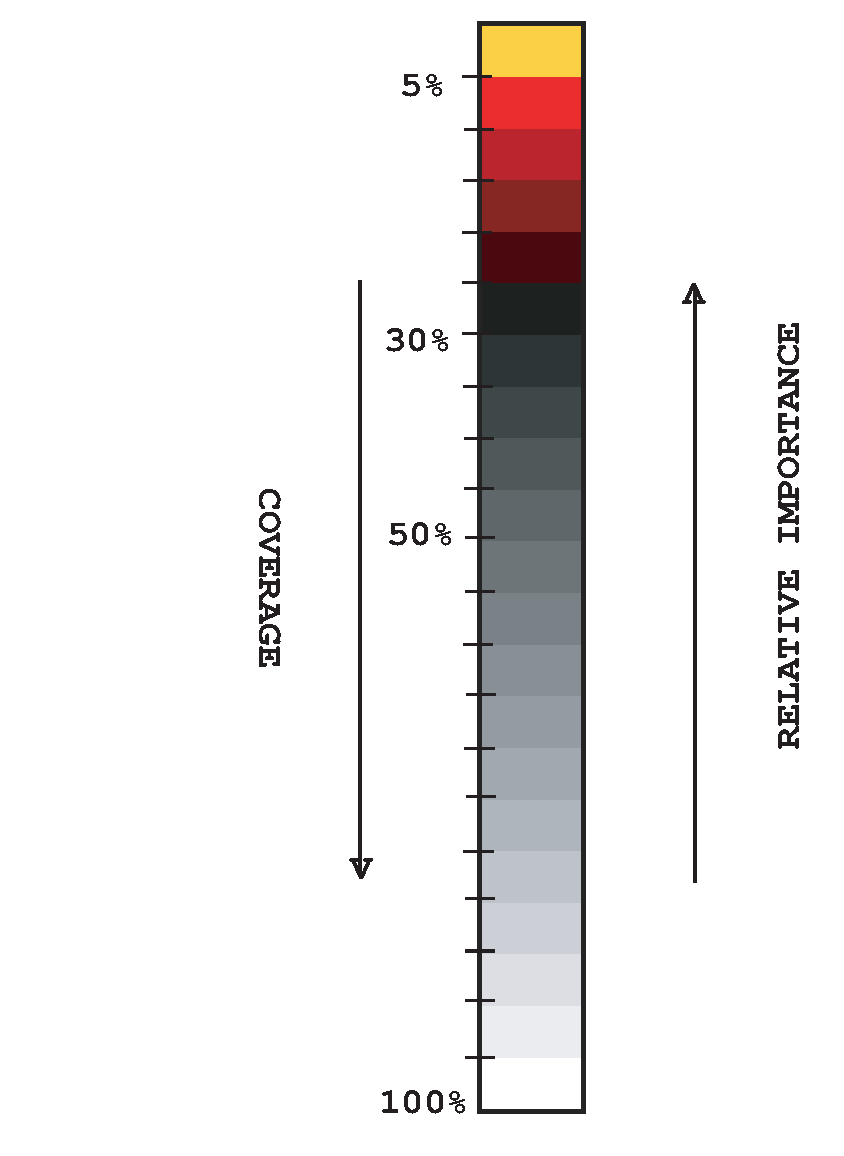
\epsfig{file=colorbar.eps,   width=0.3\linewidth}
}
\caption{\label{colorbar} Coloring scheme used to color residues by their relative importance.}
\end{figure}
The following color scheme is used in figures with residues colored by  cluster size:
 black=a single-residue cluster, clusters composed of more than one residue colored according to the hierarchy 
(ordered by descending size): red, blue, yellow, green, purple, azure, turquoise, brown, coral,
               magenta, LightSalmon, SkyBlue, violet, gold, bisque, LightSlateBlue, orchid,
               RosyBrown, MediumAquamarine, DarkOliveGreen, CornflowerBlue, grey55, burlywood,
               LimeGreen, tan, DarkOrange, DeepPink, maroon, BlanchedAlmond.

\subsection{Alistat output}
\emph{alistat} reads a multiple sequence alignment from the file, and shows a number of simple statistics about it. 
These statistics include the name of the format, the number of sequences, 
the total number of residues, the average and range of the sequence lengths, the alignment length (e.g. including gap characters).

Also shown are some percent identities. A percent pairwise alignment identity is defined as (idents / MIN(len1, len2)) 
where idents is the number of exact identities and len1, len2 are the unaligned lengths of the two sequences. 
The "average percent identity", "most related pair", and "most unrelated pair" of the alignment are the average,
 maximum, and minimum of all (N)(N-1)/2 pairs, respectively. 
The "most distant seq" is calculated by finding the maximum pairwise identity 
(best relative) for all N sequences, then finding the minimum of these N numbers (hence, the most outlying sequence). 
\emph{alistat} copyright statement:
\begin{verbatim}
HMMER 2.2g (August 2001)
Copyright (C) 1992-2001 HHMI/Washington University School of Medicine
Freely distributed under the GNU General Public License (GPL)
\end{verbatim}



\subsection{Surface accessibility according to DSSP}
 In this work a residue is considered solvent accessible if the \newline
 DSSP program (http://www.cmbi.kun.nl/gv/dssp/descrip.html) \newline
  finds it exposed to water by at least 10\AA$^2$, 
which is roughly the area  needed for one water molecule
to come in the contact with the residue.
\emph{dssp} copyright statement:
\begin{verbatim}
  W. Kabsch, C. Sander and MPI-MF, 1983, 1985, 1988, 1994 1995
  CMBI version by Elmar.Krieger@cmbi.kun.nl / November 18,2002
\end{verbatim}

\subsection{Note about ET Viewer}
 Dan Morgan from our lab has developed a visualization tool specifically for
viewing trace results. If you are interested, please visit:\newline
http://imgen.bcm.tmc.edu/molgen/labs/lichtarge/traceview/\newline
The viewer is self-unpacking and self-installing.
Input files to be used with ETV (extension .etvx) can be found in the attachment to the main report.


\subsection{Note about Rasmol/Rastop}
If you would like to visualize the results (in a clickable way) Rasmol can be found here:
http://www.bernstein-plus-sons.com/software/RasMol\_2.7.2.1.1/\newline
%
I also recommend RasTop  for Windows (unfortunately there
does not seem to be a version for Mac):
http://www.geneinfinity.org/rastop/\newline
%
%
Both applications can read the attached scripts - the files with the extension ``rs''.
On a Linux/Unix/Mac system (Rasmol)type /\newline
{\tt rasmol -script <script name> } \newline
a te the prompt. On Windows (RasTop) click in this order:  \newline
{\tt File $\rightarrow$ Open $\rightarrow$ Files of type: All Files (*)
$\rightarrow$ (select script) $\rightarrow$  Open}. \newline
